\section{Solution presentation}
\label{sec:solution}

\subsection{How to present figures}

\subsubsection{How to present just one figure}

\begin{figure}[H]
	\begin{center}
 		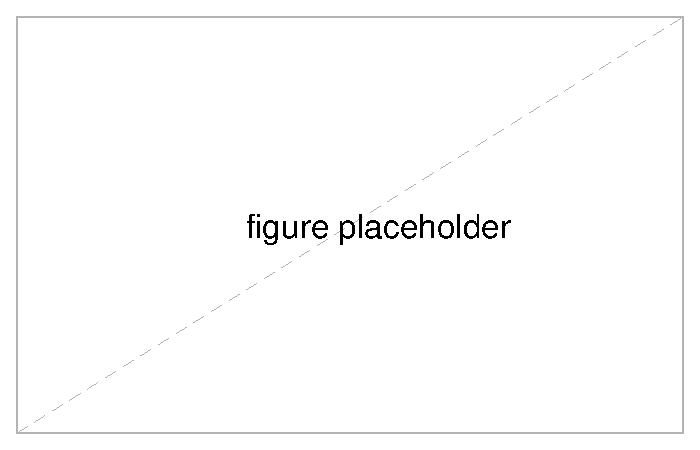
\includegraphics[width = 0.8\textwidth]{Images/Image.eps}
 		\caption{Caption}
 		\label{fig:1}
	\end{center}
\end{figure}

\subsubsection{How to present subfigures}

\begin{figure}[H]
    \centering
    \begin{subfigure}{0.33\textwidth}
        \includegraphics[width=\linewidth]{Images/Subimage1.eps}
        \caption{Subfigure 1}
        \label{fig:2.1}
    \end{subfigure}%
    \begin{subfigure}{0.33\textwidth}
        \includegraphics[width=\linewidth]{Images/Subimage2.eps}
        \caption{Subfigure 2}
        \label{fig:2.2}
    \end{subfigure}%
    \begin{subfigure}{0.33\textwidth}
        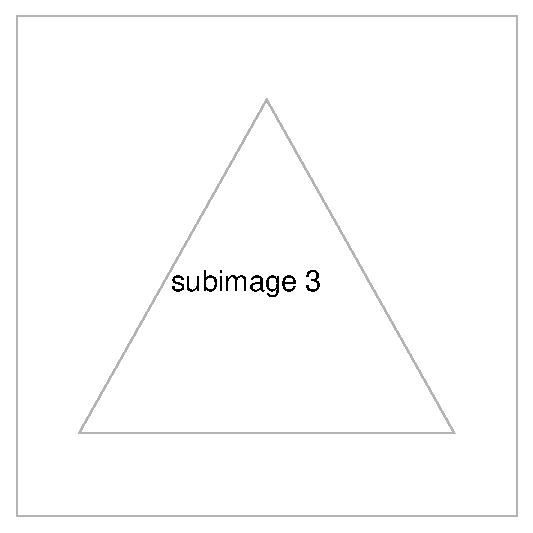
\includegraphics[width=\linewidth]{Images/Subimage3.eps}
        \caption{Subfigure 3}
        \label{fig:2.3}
    \end{subfigure}
    \caption{Caption}
    \label{fig:2}
\end{figure}

\subsection{How to present a table}

\begin{table}[H]
    \centering
    \caption{Orbital parameters for Constellation II}
    \label{tab:1}
    \begin{tabular}{|c|c|c|c|c|c|c|}
        \hline
        Satellite & $a \ [\SI{}{\meter}]$ & $e$  & $T_0$                 & $\varpi \ [\SI{}{\degree}]$ & $\Omega \ [\SI{}{\degree}]$ & $i \ [\SI{}{\degree}]$ \\ \hline
        1        & 20427.093             & 0.1 & $t_0$                 & 270                          & 0         & 60    \\ \hline
        2        & 20427.093             & 0.1 & $t_0 + \frac{T}{2}$   & 90                           & 240       & 60    \\ \hline
        3 (stat.) & 20427.093             & 0 &  N/A (circular orbit)  &  N/A (circular orbit)       & 67        & 0    \\ \hline
        4 (stat.) & 20427.093             & 0    & N/A (circular orbit) & N/A (circular orbit)       & 207       & 0     \\ \hline
    \end{tabular}
\end{table}

\subsection{How to present an equation}

\begin{equation}
    u(\lambda,T)=\frac{8\pi hc\lambda^{-5}}{e^{hc/\lambda kT}-1}
    \label{eq:1}
\end{equation}
